

\tikzset{every picture/.style={line width=0.75pt}} %set default line width to 0.75pt        

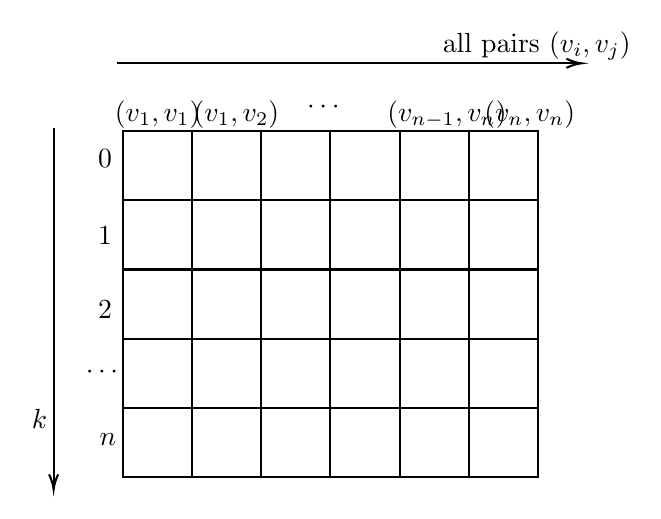
\begin{tikzpicture}[x=0.5pt,y=0.5pt,yscale=-1,xscale=1]
%uncomment if require: \path (0,370); %set diagram left start at 0, and has height of 370

%Shape: Grid [id:dp9095284515127875] 
\draw  [draw opacity=0] (87,90) -- (387,90) -- (387,340) -- (87,340) -- cycle ; \draw   (137,90) -- (137,340)(187,90) -- (187,340)(237,90) -- (237,340)(287,90) -- (287,340)(337,90) -- (337,340) ; \draw   (87,140) -- (387,140)(87,190) -- (387,190)(87,240) -- (387,240)(87,290) -- (387,290) ; \draw   (87,90) -- (387,90) -- (387,340) -- (87,340) -- cycle ;
%Straight Lines [id:da5347307434268296] 
\draw    (37,88) -- (37,347) ;
\draw [shift={(37,349)}, rotate = 270] [color={rgb, 255:red, 0; green, 0; blue, 0 }  ][line width=0.75]    (10.93,-3.29) .. controls (6.95,-1.4) and (3.31,-0.3) .. (0,0) .. controls (3.31,0.3) and (6.95,1.4) .. (10.93,3.29)   ;
%Straight Lines [id:da4989887299865372] 
\draw    (83,41) -- (416.5,41) ;
\draw [shift={(418.5,41)}, rotate = 180] [color={rgb, 255:red, 0; green, 0; blue, 0 }  ][line width=0.75]    (10.93,-3.29) .. controls (6.95,-1.4) and (3.31,-0.3) .. (0,0) .. controls (3.31,0.3) and (6.95,1.4) .. (10.93,3.29)   ;

% Text Node
\draw (67,101) node [anchor=north west][inner sep=0.75pt]   [align=left] {$\displaystyle 0$};
% Text Node
\draw (67,156.5) node [anchor=north west][inner sep=0.75pt]   [align=left] {$\displaystyle 1$};
% Text Node
\draw (67,210) node [anchor=north west][inner sep=0.75pt]   [align=left] {$\displaystyle 2$};
% Text Node
\draw (58,257.5) node [anchor=north west][inner sep=0.75pt]   [align=left] {$\displaystyle \cdots $};
% Text Node
\draw (68,306) node [anchor=north west][inner sep=0.75pt]   [align=left] {$\displaystyle n$};
% Text Node
\draw (19,289) node [anchor=north west][inner sep=0.75pt]   [align=left] {$\displaystyle k$};
% Text Node
\draw (316,16) node [anchor=north west][inner sep=0.75pt]   [align=left] {all pairs $\displaystyle ( v_{i} ,v_{j})$};
% Text Node
\draw (79,66) node [anchor=north west][inner sep=0.75pt]   [align=left] {$\displaystyle ( v_{1} ,v_{1})$};
% Text Node
\draw (346,66) node [anchor=north west][inner sep=0.75pt]   [align=left] {$\displaystyle ( v_{n} ,v_{n})$};
% Text Node
\draw (136,66) node [anchor=north west][inner sep=0.75pt]   [align=left] {$\displaystyle ( v_{1} ,v_{2})$};
% Text Node
\draw (218,66) node [anchor=north west][inner sep=0.75pt]   [align=left] {$\displaystyle \cdots $};
% Text Node
\draw (276,66) node [anchor=north west][inner sep=0.75pt]   [align=left] {$\displaystyle ( v_{n-1} ,v_{n})$};


\end{tikzpicture}

